\section{Introduction}
\frame[plain]{\sectionpage}
\addtocounter{framenumber}{-1}

\begin{frame}
  \frametitle{QCD in the dense regime}

  \vspace{.5em}

  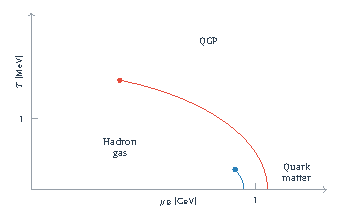
\includegraphics[width=\textwidth]{figs/phasediag.pdf}

\end{frame}

\begin{frame}
  \frametitle{The sign problem}
  \framesubtitle{Conceptual challenges}
  
  The QCD integration measure:
  \[
    \exp(\minus{}S_{\mathrm{QCD}}) = \det \qmat (\mu_B) \: \exp (\minus S_g) \tikzmark{measure}
  \]

  Monte Carlo methods rely on sampling configuration with a probability
  distribution
  \[
    P(\mathrm{conf}) \sim \exp\big(\minus{}S(\mathrm{conf})\big)
  \]
  However for \hskip5pt
  $\real (\raisebox{1pt}{$\mu_B$}) \neq 0 \,\raisebox{1pt}{$:$}$ \;%
  $\det \qmat(\raisebox{1pt}{$\mu_B$}) \in \raisebox{-1.5pt}{\scalebox{1.25}{$\mathbb{C}$}}$ 

\end{frame}

\begin{frame}
  \frametitle{The sign problem}
  \framesubtitle{Conceptual challenges}

  \vskip -.4cm

  {\centering
    \includegraphics[width=0.95\textwidth]{figs/sign_osc.pdf}
  \par}

\end{frame}

\begin{frame}
  \frametitle{The sign problem}
  \framesubtitle{Numerical approaches}

  \only<1>{
    Conventional/Monte Carlo methods:
    
    \vskip .2cm
    \begin{itemize}
    \setlength\itemsep{.5em}
      \item Reweighting
      \item Taylor expansion around $\scalemath{1.2}{\mu_B = 0}$
      \item Imaginary chemical potential
      \item Strong coupling expansions
      \item Mean field analyses
    \end{itemize}
  }

  \only<2->{
    Alternative methods:
    
    \vskip .2cm
    \begin{itemize}
    \setlength\itemsep{.5em}
      \item {\only<3>{\color{Marty}}Stochastic quantisation /
          Complex\tikzmark{langevin} Langevin}
      \item Lefschetz thimble
      \item Canonical ensembles
      \item Dual variables
      \item Density of states
    \end{itemize}
  }

  \nointerlineskip
  \begin{tikzpicture}[overlay,remember picture]
    \only<3>{
      \draw[line width=1pt,{Stealth[round]}-,Marty] ([shift={(-.1cm,-.2cm)}] langevin) -- +(0,-1.1cm)
        node[below,scale=0.8,Marty] {Current study};
    }
  \end{tikzpicture}

\end{frame}
